\chapter{Classically simulating near-term partially-distinguishable and lossy boson sampling}
\label{chp:classical_sim}

\section{Introduction}

As we saw in Chapter \ref{chp:preliminary_bs}, recent classical simulations have been expanded to consider practical issues such as photon distinguishability, based on a rich collection of theoretical work \cite{deguise2014, tamma2014, shchesnovich2014, rohde2015, shchesnovich2015, tichy2015, tillmann2015}. 
Renema et al.~\cite{renema2018} demonstrated that Boson Sampling with partially-distinguishable photons can be simulated in time which grows polynomially with $n$, which was later expanded to consider loss as well~\cite{renema2018loss}. 
However, the runtime might still not be efficient in practice, as the polynomial can be large. There is also a further disadvantage in that the error bounds are the average case for a random linear optical interferometer, meaning that there could be interferometers for which the algorithm performs significantly worse.
A significant improvement could be achieved through adapting the method of Clifford \& Clifford to this algorithm, but there are challenges with this approach.

Another motivation for adapting Clifford \& Clifford to photonic imperfection is the task of classically simulating other photonic regimes, such as Gaussian Boson Sampling \cite{hamilton2017}. The probability distribution of Gaussian Boson Sampling is that of $n$ indistinguishable squeezed states at the output of an $m$-mode linear optical interferometer, and depends on the Hafnian of a matrix. Unlike Boson Sampling, there is no known polynomial time classical algorithm for computing the probability of a single outcome from $n$ fully distinguishable squeezed states. On the other hand, it is classically efficient to sample $n$ fully distinguishable squeezed states, via a similar approach to that used for classically sampling distinguishable single photons \cite{aaronson2014}: For each squeezed state, one first samples the number of photons in that squeezed state via the inverse binomial distribution \cite{wu2019}, then each of those photons is sampled through the interferometer individually, as photons that start in the same spatial mode do not interfere with one another and their outcomes can therefore be sampled individually. As a result, adapting the Clifford \& Clifford algorithm to non-ideal Boson Sampling models provides a first step towards being able to classically simulate imperfections in Gaussian Boson Sampling.

Here we consider the cost of classically simulating Boson Sampling when the photons are partially distinguishable or lossy.
We look at the same model of distinguishability as considered in \cite{renema2018,renema2018loss}, and use techniques for modelling photon distinguishability in first quantization \cite{moylett2018, stanisic2018} to show that this is akin to choosing the indistinguishable photons of a Boson Sampling experiment via the binomial distribution. 
We combine this with the well-studied model of uniform loss, where each photon independently survives with probability $\eta$. Under this model, the probability of how many photons survive overall also follows a binomial distribution. 
This gives rise to a method which is able to naturally apply the Clifford \& Clifford algrithm and take advantage of its efficiency. This algorithm also offers a worst-case error bound for \textit{any} linear optical interferometer, rather than a random one.
Although this approach only offers a polynomial improvement compared to the runtime for ideal Boson Sampling (unlike the exponential improvement shown in \cite{renema2018,renema2018loss}) we use analytical bounds to show that for photon numbers of experimental interest our algorithm can make a significant improvement over alternative approaches. 

This chapter is laid out as follows.
In Section \ref{sec:expansion}, we show what the Renema et al.~\cite{renema2018, renema2018loss} model of distinguishability looks like in first quantization, and provide an alternative classical simulation. 
In Section \ref{sec:average-case}, we consider average error bounds for a Haar-random unitary interferometer, via the methods explained in Section \ref{sec:renema-review}. 
In Section \ref{sec:worst-case}, we improve this bound to a worst-case error bound, by computing an upper bound for the trace distance between our approximation and the model. 
In Section \ref{sec:loss}, we expand these results to consider uniform loss, and show how distinguishability and loss relate to each other. 
In Section \ref{sec:empirical-errors}, we explore these error bounds for experimentally interesting numbers of photons, and show that there are some cases where our algorithm offers an improvement. 
Finally, we briefly consider \emph{non}-uniform loss, where loss is a function of the number of optical components, and use the methods of \cite{garciapatron2017, oszmaniec2018} to show that classical simulations with non-uniform loss also become easier when distinguishability is introduced.
We conclude with some open research questions in Section \ref{sec:conclusion}.

\section{Limitations of other classical simulation algorithms}

Before disucssing our classical algorithm, we shall look at other classical potential classical simulation algorithms and explain some of their limitations when applied to Boson Sampling under distinguishability. In particular, we shall discuss adapting the methods of \cite{havlicek2018, havlicek2019} and \cite{oszmaniec2018} to Boson Sampling under distinguishability and loss.

\subsection{Classical Tractability}

We shall start by discussing the issue with employing the Classical Tractability method of Van den Nest \cite{vandennest2011}, similarly to the technique used by Havl\'{i}\v{c}ek and Strelchuk \cite{havlicek2018}. There are some promising initial results for using this technique to approximate the transition amplitudes of imperfect Boson Sampling, but it very quickly becomes clear that this is not efficiently possible in general.

Recall from Section \ref{ssec:schur-simulation} that a state is Classically Tractable if we can efficiently approximate its amplitudes and sample from measuring the state in the computational basis up to polynomial multiplicative error \cite{vandennest2011}. It is easy to see in this case that the input state to Boson Sampling in the first quantisation is a CT state, as the only basis states with non-zero amplitude are those which are permutations of $[n]$, and those states have uniform amplitudes. More formally, the amplitude of a state $\ket{a}\in(\mathbb{C}^m)^{\otimes n}$ is

\begin{equation}
\psi_a = \begin{cases}1/\sqrt{n!} & \quad \textrm{if } \exists \sigma\in\symm_n \textrm{ s.t. } \sigma(a_i) = i \forall i\in[n]\\0 & \quad{otherwise}\end{cases}.
\end{equation}

Similarly, a measurement in the computational basis can be efficiently sampled by sampling a permutation $\sigma \in \symm_n$ uniformly at random and outputting $\sigma(1), \sigma(2),\dots,\sigma(n)$. Thus our input state meets the requirements for Computational Tractability.

This seems promising, as the entanglement was believed to be the hard part of Section \ref{sec:mixture}, and now this provides a way of classically simulating that step. However, we shall see that in this setting the action of the interferometer leads to classical simulation being hard.

In order to approximate the probability of an outcome, the operation we apply to the input state needs to be Efficiently Computable Sparse (ECS). From Van den Nest \cite{vandennest2011}, this means that each row and column of the matrix has at most $\poly(n)$ non-zero elements and each element of the matrix can be approximated to polynomial multiplicative error in polynomial time. In our case, this operator is $U^{\otimes n}$.

Each element of this operator can be efficiently approximated as a product of different elements of $U$. However, the matrix is very large, with $m^n$ elements in each row and column. This is especially poor in the case where $m = O(n^2)$, believed to be the regime required for Boson Sampling to provide a quantum advantage.

There are some potentially positive directions in this area. If there are a small number of non-zero elements in each row and column of $U$, then many of the elements in $U^{\otimes n}$ would also be zero, and then the matrix could be interpreted as ECS. This could be true if, for example, the photonic circuit is low depth. Another potential direction is to use this method to simulate Boson Sampling under photon loss, which would reduce the exponent. However, it is unclear how either of these methods would lead to a faster simulation than ones that are already known.

\subsection{Distance from the fully distinguishable state}
\label{ssec:fixed-dist-distance}

In this section we shall consider limitations with simply using a separable state. This is inspired by the work on Oszmaniec and Brod \cite{oszmaniec2018}, who showed that with sufficient amounts of loss the Boson Sampling input state is arbitrarily close to a known separable state. However, it is also similar to the technique used by Deshpande et al.~\cite{deshpande2018} and Maskara et al.~\cite{maskara2019}, who used the input state of fully distinguishable particles to classically simulate Boson Sampling with low-depth circuits.

The most natural state to use to classically simulate Boson Sampling under distinguishability is the fully distinguishable state

\begin{equation}
\rho_D = \frac{1}{n!}\sum_{\sigma\in\symm_n}\sigma\ket{s}\bra{s}\sigma^\dagger,
\end{equation}

\noindent where $\ket{s} = \bigotimes_{i=1}^n\ket{i}$. We shall also use 

\begin{equation}
\rho_I = \sum_{\sigma, \sigma' \in \symm_n}\sigma\ket{s}\bra{s}\sigma'^\dagger
\end{equation}

\noindent to indicate the fully indistinguishable input state.

As already noted in Section \ref{ssec:fully-dist-sim}, this state is completely separable, and an interferometer acting on it can be classically simulated in polynomial time. In this section, we shall compute the trace distance between this state and various other Boson Sampling input states which could be interesting. For this, note that the trace distance between mixed states $\rho, \rho'$ is defined as

\begin{equation}
\delta_{\trace}
(\rho, \rho') = \trace(\sqrt{(\rho - \rho')(\rho-\rho')^\dagger}).
\end{equation}

We start by subtracting $\rho_I$ from $\rho_D$, which gives the matrix\begin{align}
\rho_I - \rho_D &= \frac{1}{n!}\left(\sum_{\sigma,\sigma'\in\textrm{S}_n}\sigma\ket{s}\bra{s}\sigma'^\dagger - \sum_{\sigma \in \textrm{S}_n}\sigma\ket{s}\bra{s}\sigma^\dagger\right)\\
&= \frac{1}{n!}\left(\sum_{\substack{\sigma,\sigma'\in\textrm{S}_n\\\sigma\neq\sigma'}}\sigma\ket{s}\bra{s}\sigma'^\dagger\right).
\end{align}

Multiplying this matrix by its Hermitian adjoint gives the positive semidefinite matrix

\begin{align}
(\rho_I - \rho_D)(\rho_I - \rho_D)^\dagger &= \frac{1}{(n!)^2}\left(\sum_{\substack{\sigma,\sigma'\in\textrm{S}_n\\\sigma\neq\sigma'}}\sigma\ket{s}\bra{s}\sigma'^\dagger\right)\left(\sum_{\substack{\tau,\tau'\in\textrm{S}_n\\\tau\neq\tau'}}\tau'\ket{s}\bra{s}\tau^\dagger\right)\\
&= \frac{1}{(n!)^2}\left((n! - 2)\sum_{\sigma,\tau\in\textrm{S}_n}\sigma\ket{s}\bra{s}\tau^\dagger + \sum_{\sigma \in \textrm{S}_n}\sigma\ket{s}\bra{s}\sigma^\dagger\right).
\end{align}

As the above matrix is positive semidefinite, we can find its square root as

\begin{align}
\sqrt{(\rho_I - \rho_D)(\rho_I - \rho_D)^\dagger} &= \frac{1}{n!}\left(\left(\frac{n!-2}{n!}\right)\sum_{\sigma,\tau\in\textrm{S}_n}\sigma\ket{s}\bra{s}\tau^\dagger + \sum_{\sigma \in \textrm{S}_n}\sigma\ket{s}\bra{s}\sigma^\dagger\right).
\end{align}

From this we can work out the trace difference between the two states to be

\begin{align}
\delta_{\mathrm{tr}}(\rho_I, \rho_D) &= \frac{1}{2\times n!}\left(\left(\frac{n!-2}{n!}\right)n! + n!\right)\\
&= \frac{1}{2}\left(\frac{n!-2}{n!} + 1\right)\\
&= \frac{2 \times n! - 2}{2 \times n!}\\
&= 1 - \frac{1}{n!}.
\end{align}

We next consider the singly distinguishable state, as considered by Stanisic and Turner \cite{stanisic2018}. If we denote the distinguishable photon as the photon in mode $i$, the first quantisation state looks like

$$\rho_{SD} = \frac{1}{n!}\sum_{\substack{\sigma,\sigma'\in\textrm{S}_n\\\sigma^{-1}(i)=\sigma'^{-1}(i)}}\sigma\ket{s}\bra{s}\sigma'^\dagger.$$

Following the same structure as with fully indistinguishable photons, we find that subtracting the two matrices gives

\begin{align}
\rho_{SD} - \rho_D &= \frac{1}{n!}\left(\sum_{\substack{\sigma,\sigma'\in\textrm{S}_n\\\sigma^{-1}(i)=\sigma'^{-1}(i)}}\sigma\ket{s}\bra{s}\sigma'^\dagger - \sum_{\sigma \in \textrm{S}_n}\sigma\ket{s}\bra{s}\sigma^\dagger\right)\\
&= \frac{1}{n!}\left(\sum_{\substack{\sigma,\sigma'\in\textrm{S}_n\\\sigma^{-1}(i)=\sigma'^{-1}(i)\\\sigma\neq\sigma'}}\sigma\ket{s}\bra{s}\sigma'^\dagger\right).
\end{align}

Multiplying the matrix by its adjoint gives the positive semidefinite matrix

\begin{align}
(\rho_{SD} - \rho_D)(\rho_{OBE} - \rho_D)^\dagger &= \frac{1}{(n!)^2}\left(\sum_{\substack{\sigma,\sigma'\in\textrm{S}_n\\\sigma^{-1}(i)=\sigma'^{-1}(i)\\\sigma\neq\sigma'}}\sigma\ket{s}\bra{s}\sigma'^\dagger\right)\left(\sum_{\substack{\tau,\tau'\in\textrm{S}_n\\\tau^{-1}(i)=\tau'^{-1}(i)\\\tau\neq\tau'}}\tau'\ket{s}\bra{s}\tau^\dagger\right)\\
&= \frac{1}{(n!)^2}\left(((n-1)! - 2)\sum_{\substack{\sigma,\tau\in\textrm{S}_n\\\sigma^{-1}(i)=\tau^{-1}(i)}}\sigma\ket{s}\bra{s}\tau^\dagger + \sum_{\sigma \in \textrm{S}_n}\sigma\ket{s}\bra{s}\sigma^\dagger\right).
\end{align}

We can then work out the square root of this positive semidefinite matrix as the positive matrix

\begin{align}
\sqrt{(\rho_{OBE} - \rho_D)(\rho_{OBE} - \rho_D)^\dagger} &= \frac{1}{n!}\left(\left(\frac{(n-1)!-2}{(n-1)!}\right)\sum_{\substack{\sigma,\tau\in\textrm{S}_n\\\sigma^{-1}(i)=\tau^{-1}(i)}}\sigma\ket{s}\bra{s}\tau^\dagger + \sum_{\sigma \in \textrm{S}_n}\sigma\ket{s}\bra{s}\sigma^\dagger\right).
\end{align}

Finally, we work out the trace of this matrix, and find the trace distance to be

\begin{align}
\delta_{\mathrm{tr}}(\rho_{SD}, \rho_D) &= \frac{1}{2\times n!}\left(\left(\frac{(n-1)!-2}{(n-1)!}\right)n! + n!\right)\\
&= \frac{1}{2}\left(\frac{(n-1)!-2}{(n-1)!} + 1\right)\\
&= \frac{2 \times (n-1)! - 2}{2 \times (n-1)!}\\
&= 1 - \frac{1}{(n-1)!}.
\end{align}

An intuitive question to ask at this point is to make sure this distance still applies after applying the Schur transform again, thus matching the method used by Stanisic and Turner \cite{stanisic2018}.

The fully distinguishable state in this picture is

\begin{equation}
\rho_D = \frac{1}{n!} \sum_{\lambda \vdash n} \sum_{q_\lambda^\mathrm{coin}} \sum_{p_\lambda} |\lambda,p_\lambda,q_\lambda\rangle\langle \lambda,p_\lambda,q_\lambda|.
\end{equation}

Depending on choice of Schur basis, we can describe the Singly Distinguishable state as

\begin{equation}
\rho_{SD} = \frac{1}{n}\left(\ket{(n),1,\underline{1},1}\bra{(n),1,\underline{1},1} + \sum_{p}\ket{(n-1,1),p,\underline{1},1}\bra{(n-1,1),p,\underline{1},1}\right),
\end{equation}

\noindent where we have written $q_\lambda$ as an occupation number and multiplicity.

The terms in the singly distinguishable case have amplitudes of $(1/n!)$ in the fully distinguishable case, so these terms will be $1-n - 1/n! = ((n-1)!-1)/n!$ in the difference matrix, with other diagonal terms having $0$ apart from $n!-n$ which appear in $\rho_D$ but not in $\rho_{SD}$, which have value $1/n!$. The trace distance thus ends up being

\begin{align}
\delta_{\mathrm{tr}}(\rho_{OBE},\rho_{D}) &= \frac{1}{2}\left(\frac{(n-1)!-1}{n!}\times n + \frac{n!-n}{n!}\right)\\
&= \frac{1}{2}\left(2\times\frac{n!-n}{n!}\right)\\
&= \frac{n!-n}{n!}\\
&= 1 - \frac{1}{(n-1)!}.
\end{align}

Therefore either technique produces the same trace distance.

We can easily generalise the two results above to a case where $k$ photons are fully indistinguishable, and the remaining $n-k$ are fully distinguishable. Now we specify that $\sigma^{-1}(i)=\sigma'^{-1}(i)\forall i \in \bar{K}$, where $\bar{K}$ is the set of $n-k$ distinguishable photons. The only other change is that the $(n-1)!$ terms become $k!$. The final trace distance will be $1-1/k!$. Even more generally, it seems likely that if we have two states with indistinguishable photons defined by set $K$ and $K'$, then the trace distance would equal $|K\cap K'|!/|K\cap K'|!$, though this has not been formally proven.

As can be seen from the above, for $k$ indistinguishable photons and $n-k$ photons which are fully distinguishable from every other photon, we have the trace distance $\delta_{\mathrm{tr}}$ reducing as $1 - 1/k!$.

The property which the trace distance is useful for is that it is an upper bound of the total variation distance. According to Oszmaniec and Brod, this is helpful for loss as the trace distance tends to $0$ as more photons are lost. But even when only two photons are indistinguishable, we still have a trace distance of $1/2$, and this error only increases with the number of indistinguishable photons.

We shall conclude this section by considering a somewhat more positing case: the state $\rho_\epsilon$, as described in Equation \ref{eq:Werner} from Section \ref{sec:mixture}:

\begin{equation}
\rho_\epsilon = (1-\epsilon)\rho_D + \epsilon\rho_I.
\end{equation}

The trace distance between this state and the fully distinguishable state is

\begin{align}
\delta_{\textrm{tr}}(\rho_\epsilon,\rho_D) &\leq (1-\epsilon)\delta_{\textrm{tr}}(\rho_D,\rho_D) + \delta_{\textrm{tr}}(\epsilon\rho_I,\rho_D)\\
&= \epsilon-\frac{\epsilon}{n!},
\end{align}

\noindent where we have used the fact that the trace distance in convex. Noting that $\lim_{n\rightarrow\infty}\epsilon/n! = 0$, we can conclude that as $n\rightarrow\infty$ this state tends to $\epsilon$. This is an interesting change from the previous sections, but not particularly surprising, given that we are asking for the classical part of the state to essentially dominate the result.

\section{Expanding in terms of states}
\label{sec:expansion}

We will now introduce a new expression for partially distinguishable particles. We start by writing the input state of $n$ photons, with pairwise distinguishability parameter $x$ as in the previous section, in first quantization
\begin{equation}
\label{eqn:rhon}
\rho_{n,x} = \frac{1}{n!}\left(\sum_{\sigma,\sigma'\in\symm_n}\sigma\ket{s}\bra{s}\sigma'x^{\sigma\cdot\sigma'}\right),
\end{equation}
where we have used $\sigma\cdot\sigma'$ to denote the number of places where permutations $\sigma$ and $\sigma'$ match.
For reference, the expansion of \cite{renema2018,renema2018loss} is carried out by identifying $\sigma$ and $\sigma'$ that match for a fixed set of $i$ points:
\begin{equation}
\label{eqn:rhoni}
\rho_{n,x} = \frac{1}{n!}\left(\sum_{i=0}^nx^i\sum_{\substack{\sigma,\sigma'\in\symm_n\\\exists I\subseteq [n] \textrm{ s.t. } |I|=i\\\sigma^{-1}(j)\neq\sigma'^{-1}(j)\forall j \in I\\\sigma^{-1}(j)=\sigma'^{-1}(j)\forall j \notin I}}\sigma\ket{s}\bra{s}\sigma'^\dagger\right).
\end{equation}
Note here that the terms in the sum over permutations do not correspond to physical states. 
This can be seen by the fact that for $i\neq 0$ this summation has no elements along the diagonal of the density matrix, as $\sigma$ and $\sigma'$ need to differ in \emph{exactly} $i$ places.

We instead look at an alternative expansion, in order to decompose the model into a linear combination of physical states:
\begin{align}
\rho_{n,x} &= \frac{1}{n!}\left(\sum_{i=0}^np_i\sum_{\substack{\sigma,\sigma'\in\symm_n\\\exists I\subseteq [n] \textrm{ s.t. } |I|=i\\\sigma^{-1}(j)=\sigma'^{-1}(j)\forall j \notin I}}\sigma\ket{s}\bra{s}\sigma'^\dagger\right)\label{eqn:state-expansion}\\
&= \sum_{i=0}^np_i\sum_{\substack{I\subseteq[n]\\|I|=i}}\left(\frac{1}{n!}\sum_{\substack{\sigma,\sigma'\in\symm_n\\\sigma^{-1}(j)=\sigma'^{-1}(j)\forall j \notin I}}\sigma\ket{s}\bra{s}\sigma'^\dagger\right)\\
&= \sum_{i=0}^np_i\sum_{\substack{I\subseteq[n]\\|I|=i}}\rho_I, \label{eq:newrho}
\end{align}
where $\rho_I$ is the state where photons in modes $j \in I$ are fully indistinguishable from each other, all other photons are fully distinguishable, and $0 \leq p_i \leq 1$ is a coefficient dependent on $x$ and $n$ determining the probability of a state with $i$ indistinguishable single photons.

Note that unlike Equation (\ref{eqn:rhoni}), where permutations must differ in exactly $i$ points, in Equation (\ref{eqn:state-expansion}) we allow permutations to differ in \emph{at most} $i$ points. 
This means that elements closer to and along the diagonal of the density matrix are also part of this summation, and this means that each $\sigma,\sigma' \in \symm_n$ term forms a valid density matrix.

Already we can see how a classical simulation might work -- if we are able to sample $p_i$ efficiently, then we can choose $\rho_I$ by selecting $i$ photons uniformly at random to be indistinguishable. 
These $i$ photons can be classically simulated using Clifford \& Clifford \cite{clifford2017}, while the remaining $n-i$ photons are treated as fully distinguishable photons, each of which can be simulated individually in polynomial time \cite{aaronson2014,neville2017}.


\subsection{The $p_i$ are binomially distributed}
\label{sec:understanding-pi}

Here, we will show that the coefficients $p_i$ follow the binomial distribution
\begin{equation}
p_i = x^i(1-x)^{n-i}.
\end{equation}

%To start, it is not hard to see that coefficients $p_i$ following the binomial distribution gives a state with trace $1$, ensuring validity:
%\begin{align}
%\trace[\rho_{n,x}] &= \sum_{i=0}^nx^i(1-x)^{n-i}\sum_{\substack{I\subseteq[n]\\|I|=i}}\trace[\rho_I]\\
%&= \sum_{i=0}^nx^i(1-x)^{n-i}\sum_{\substack{I\subseteq[n]\\|I|=i}}1\\
%&= \sum_{i=0}^nx^i(1-x)^{n-i}\binom{n}{i}\\
%&= (x + 1 - x)^n\\
%&= 1.
%\end{align}
%As the trace is the sum of diagonal elements in the density matrix, we can conclude that all elements along the diagonal of the density matrix are $1/n!$, agreeing with Eq.~(\ref{eq:}).
%{\blue I now don't think that this really shows anything other than the fact the binomial distribution is 

To see that the matrix elements of Eq.~(\ref{eq:newrho}) with $p_i$ binomially distributed equal those of Eq.~(\ref{eqn:rhoni}), consider  $\sigma,\sigma'$ which differ at points in the set $I$, where $|I|=i$; the coefficient here should be $x^i$.
Contributing to this element of the density matrix will be the state $\rho_I$, as well as other states $\rho_{I'}$, where $I \subseteq I'$. 
The number of such sets $I'$ is $\binom{n-i}{i'-i}$, as it is equivalent to choosing $i'$ from $n$ elements when $i$ elements have already been chosen. 
The corresponding matrix element is
%\begin{widetext}
\begin{align}
&\frac{1}{n!}\left(\sum_{{i'}=i}^n x^{i'}(1-x)^{n-{i'}}\binom{n-i}{{i'}-i}\right) \\
&= \frac{1}{n!}\left(x^i\sum_{{i'}=i}^n x^{{i'}-i}(1-x)^{n-{i'}}\binom{n-i}{{i'}-i}\right)\\
&= \frac{1}{n!}\left( x^i\sum_{{i'}=0}^{n-i}x^{i'}(1-x)^{n-i-{i'}}\binom{n-i}{{i'}}\right)\\
&= \frac{x^i(x + 1 - x)^{n-i}}{n!}\\
&= \frac{x^i}{n!}.
\end{align}
%\end{widetext}
%Here the first thing we have done is to remove a common factor of $x^i$, followed by relabelling $j$ to sum from $0$ to $n-i$. After that we have applied the binomial theorem and cancelled terms as with the trace to get the correct value. 
It is not hard to see that the state is normalised
\begin{align}
\trace[\rho_{n,x}] &= \sum_{i=0}^nx^i(1-x)^{n-i}\sum_{\substack{I\subseteq[n]\\|I|=i}}\trace[\rho_I]\\
&= \sum_{i=0}^nx^i(1-x)^{n-i}\sum_{\substack{I\subseteq[n]\\|I|=i}}1\\
&= \sum_{i=0}^nx^i(1-x)^{n-i}\binom{n}{i}\\
&= (x + 1 - x)^n\\
&= 1.
\end{align}
%We have therefore shown that any elements in the density matrix describing our state match the corresponding element in the state of \ref{eqn:rhoni}.
Thus this model of fixed pairwise distinguishability can be written as an expansion in terms of valid states, where indistinguishable photons are drawn from a binomial distribution.


\subsection{Classical simulation} %via truncation of indistinguishable photons}

We can now see explicitly how a simulation for Boson Sampling with distinguishable photons would work. 
First, we sample an integer $i \in [n]$ according to the Binomial distribution with coefficients $n$ and $x$. 
Next, we sample a subset $I$ of the photons uniformly at random from the $\binom{n}{i}$ possible subsets of size $i$. 
These are the indistinguishable photons of our simulation, which we simulate using Clifford and Clifford in $O(i2^i + \poly(i,m))$ time. 
The remaining $n-i$ photons are considered to be distinguishable. 
Rather than needing to compute the output probabilities of these photons collectively, which could take between $O(n-i)^4\log(n-i)$ and $O(n-i)^7\log^4(n-i)$ time via permanents of matrices with non-negative entries \cite{huber2008}, we can instead sample each distinguishable photon individually. 
To do so, we take a distinguishable photon in mode $a$, and compute the probability of this photon being measured in mode $b$ as $|U_{b,a}|^2$. 
Thus we can compute all output probabilities and obtain a sample for a single distinguishable photon in $O(m)$ time, meaning that we can obtain a sample for all $n-i$ distinguishable photons in $O(m(n-i))$ time \cite{aaronson2014,neville2017}.

The run time is dominated by the time taken to sample our indistinguishable photons, which can be as large as $O(n2^n + \poly(n,m))$ if we are unlucky. 
By truncating our binomial sampling up to some level $k$, we can simulate Boson Sampling up to some level of error. 
The extent of this error will be the focus of Secs. \ref{sec:average-case} \& \ref{sec:worst-case}.



\section{Average case error}
\label{sec:average-case}

We can use the same strategies used in \cite{renema2018,renema2018loss} to derive an error bound for Boson Sampling via state truncation for a Haar-random interferometer. We shall do this by considering the expected total variation distance between our approximation and the model for partial distinguishability for a Gaussian matrix. This is given by

\begin{align}
\mean[\Delta P] &= \mean\left[\frac{1}{2}\sum_{S'}|\prob[S']-\prob_k[S']|\right]\\
&= \frac{1}{2}\sum_{S'}\mean|\prob[S']-\prob_k[S']| \label{eqn:tvd},
\end{align}
where $\prob_k$ is the probability distribution truncated at $k$ indistinguishable photons via our approximation. For a specific outcome $S'$, we can expand the right hand side to
\begin{align}
\mean\left[|\prob[S']-\prob_k[S']|\right] = &\mean\left|\sum_{i=0}^k\left(p_i-p_i'\right)\sum_{\substack{I\subseteq[n]\\|I|=i}}P_I[S']+\sum_{i=k+1}^np_i\sum_{\substack{I\subseteq[n]\\|I|=i}}P_I[S']\right|,
\end{align}
where $P_I$ is now the probability distribution with indistinguishable photons defined by set $I$, and $p_i'=p_i/(\sum_{i=0}^kx^i(1-x)^{n-i}\binom{n}{i})$ is the normalised version of the $p_i$ coefficients defined in Section \ref{sec:expansion}. 
Note that $P_I$ is the distribution arising from state $\rho_I$ in Section \ref{sec:expansion}. 
We can use the triangle inequality to bound this value to
\begin{align}
\mean\left[|\prob[S']-\prob_k[S']|\right] &\leq \mean\left|\sum_{i=0}^k\left(p_i-p_i'\right)\sum_{\substack{I\subseteq[n]\\|I|=i}}P_I[S']\right|+\mean\left|\sum_{i=k+1}^np_i\sum_{\substack{I\subseteq[n]\\|I|=i}}P_I[S']\right|\\
&= \mean[\Delta P_{\leq k}] +\mean[\Delta P_{> k}]\label{eqn:single-outcome-error},
\end{align}
where we have introduced variables $\Delta P_{\leq k}$ and $\Delta P_{> k}$ for convenience. 
We shall consider the expected values of these terms for a Gaussian matrix separately, starting with the latter.
Using the Laplace expansion, we find that
\begin{align}
\mean[\Delta P_{>k}] &= \sum_{i=k+1}^np_i\sum_{\substack{I\subseteq[n]\\|I|=i}}\mean\left[P_I[S']\right],\\
&=\sum_{i=k+1}^np_i\sum_{\substack{I\subseteq[n]\\|I|=i}}\sum_{\substack{J\leq S'\\|J|=i}}\mean\left[|\per(U_{I,J})|^2\per(|U_{\bar{I},\bar{J}}|^2)\right],\label{eqn:laplace}
\end{align}
where $U_{I,J}$ is a matrix defined from our interferometer $U$ by selecting columns according to $I$ and rows according to $J$, and $|U_{\bar{I}\bar{J}}|^2$ is a matrix whose elements are the absolute values squared of $U_{\bar{I},\bar{J}}$.

We next need to consider the expected values of the matrix permanents in Equation (\ref{eqn:laplace}) for a Haar random unitary. 
To do this, we shall assume the matrix describing our interferometer is Gaussian. 
This allows us to assume that each entry of $U_{I,J}$ and $|U_{\bar{I},\bar{J}}|^2$ is independent, and that the two matrices are independent of each other. 
Starting with $\per(|U_{\bar{I},\bar{J}}|^2)$, we note that this is a Gaussian matrix of size $(n-i)\times(n-i)$, and each entry is the square of two independent Gaussians, meaning that each entry of $|U_{\bar{I},\bar{J}}|^2$ has expected value $1/m$. 
From this, we can calculate the expected value as
\begin{equation}
\mean[\per(|U_{\bar{I},\bar{J}}|^2)] = \frac{(n-i)!}{m^{n-i}}.
\end{equation}

For $U_{I,J}$, we note that each element of $U_{I,J}$ is an independent Gaussian entry, with mean value $0$ due to symmetry, and second order moment $\mean[|U_{i,j}|^2] = 1/m$. The second order moment for the permanent can then be calculated using the same methods as in \cite{aaronson2011}:
\begin{align}
\mean[|\per(U_{I,J})|^2] &= \mean\left[\sum_{\sigma,\sigma'\in\symm_i}\prod_{l=1}^n(U_{I,J})_{l,\sigma(l)}(U^*_{I,J})_{l,\sigma'(l)}\right]\\
&= \mean\left[\sum_{\sigma\in\symm_i}\prod_{l=1}^n|(U_{I,J})_{l,\sigma(l)}|^2\right]\\
&= \sum_{\sigma\in\symm_i}\prod_{l=1}^n\mean\left[|U_{l,\sigma(l)}|^2\right]\\
&= \frac{i!}{m^{i}}.
\end{align}
Because the two matrices are independent~\cite{renema2018}, we can express the expected value of their product as
\begin{align}
\mean\left[|\per(U_{I,J})|^2\per(|U_{\bar{I},\bar{J}}|^2)\right] &= \frac{(n-i)!}{m^{n-i}}\times\frac{i!}{m^{i}}\\
&= \frac{(n-i)!i!}{m^n}.
\end{align}
Plugging this into Equation (\ref{eqn:laplace}), we find that
\begin{align}
\mean[\Delta P_{>k}] &= \sum_{i=k+1}^np_i\sum_{\substack{I\subseteq[n]\\|I|=i}}\sum_{\substack{J\leq S'\\|J|=j}}\frac{(n-i)!i!}{m^n}\\
&= \sum_{i=k+1}^np_i\binom{n}{i}^2\frac{(n-i)!i!}{m^n}\\
&= \frac{n!}{m^n}\sum_{i=k+1}^np_i\binom{n}{i}\\
&= \frac{n!}{m^n}\sum_{i=k+1}^nx^i(1-x)^{n-i}\binom{n}{i},
\end{align}
where first we use the fact that since our input and output are both collision-free, there are $\binom{n}{i}$ ways of choosing $I$ and $J$, then apply cancellation, and finally substitute the values of $p_i$. 
This gives our error bound for terms not in our approximation.

Next we shall consider the term $\Delta P_{\leq k}$. 
First we can note that $p_i' \geq p_i \forall i\leq k$, due to the normalisation of $p_i'$. 
Thus we can rewrite this term as
\begin{align}
\mean[\Delta P_{\leq k}] &= \sum_{i=0}^k(p_i'-p_i)\sum_{\substack{I\subseteq[n]\\|I|=i}}\mean\left[P_I[S']\right].
\end{align}
Using the same techniques for computing the Laplace expansion and calculating the expected value of permanents of Gaussian matrices, we can show that
\begin{align}
\mean[\Delta P_{\leq k}] &= \sum_{i=0}^k(p_i'-p_i)\binom{n}{i}^2\frac{(n-i)!i!}{m^n}\\
&= \frac{n!}{m^n}\sum_{i=0}^k(p_i'-p_i)\binom{n}{i}\label{eqn:gtk}.
\end{align}

Next we expand $p_i'$:
\begin{align}
\sum_{i=0}^kp_i'\binom{n}{i} &= \frac{\sum_{i=0}^kx^i(1-x)^{n-i}\binom{n}{i}}{\sum_{i=0}^kx^i(1-x)^{n-i}\binom{n}{i}}\\
&= 1,
\end{align}
and use this expansion as well as the value of $p_i$ to calculate
\begin{align}
\mean[\Delta P_{\leq k}] &= \frac{n!}{m^n}\left(1 - \sum_{i=0}^kx^i(1-x)^{n-i}\binom{n}{i}\right)\\
&= \frac{n!}{m^n}\sum_{i=k+1}^nx^i(1-x)^{n-i}\binom{n}{i}\label{eqn:leqk}.
\end{align}

We plug our values for Equations \ref{eqn:gtk} \& \ref{eqn:leqk} into Equation \ref{eqn:single-outcome-error} to bound our error for a single outcome as

\begin{equation}
\mean\left[|\prob[S']-\prob_k[S']|\right] \leq 2\frac{n!}{m^n}\sum_{i=k+1}^nx^i(1-x)^{n-i}\binom{n}{i}.
\end{equation}

Finally, we use these values and sum over all collision-free $S'$, of which there are $\binom{m}{n}\approx m^n/n!$ to bound the expectation of our total variation distance for a Haar-random unitary as

\begin{align}
\mean[\Delta P] &\leq \frac{1}{2}\sum_{S'}2\frac{n!}{m^n}\sum_{i=k+1}^nx^i(1-x)^{n-i}\binom{n}{i}\\
&\approx \frac{m^n}{n!}\frac{n!}{m^n}\sum_{i=k+1}^nx^i(1-x)^{n-i}\binom{n}{i}\\
&=\sum_{i=k+1}^nx^i(1-x)^{n-i}\binom{n}{i}.
\end{align}

It seems like there should be some room for improvement in this bound. 
In particular, the use of the triangle inequality suggests that there might be more precise approximations of the expected distance.

\section{Worst case error}
\label{sec:worst-case}

We shall now use a different technique to show that the above Haar average case error bound matches the worst-case error for any linear-optical interferometer. We do so by finding an upper bound for the trace distance between our ideal partially distinguishable state and the approximation that results from truncating at some $k$, the size of the largest indistinguishable set of particles.
As the trace distance is an upper bound for any POVM measurement, we know that this will provide an upper bound for the difference in distribution produced by any interferometer.

Denoting our truncated state
\begin{equation}
\rho_{\leq k,x} = \frac{\sum_{i=0}^kx^i(1-x)^{n-i}\sum_{\substack{I\subseteq[n]\\|I|=i}}\rho_I}{\sum_{i=0}^kx^i(1-x)^{n-i}\binom{n}{i}},
\end{equation}
where the denominator is a normalising factor, and similarly
\begin{equation}
\rho_{>k,x} = \frac{\sum_{i=k+1}^nx^i(1-x)^{n-i}\sum_{\substack{I\subseteq[n]\\|I|=i}}\rho_I}{\sum_{i=k+1}^nx^i(1-x)^{n-i}\binom{n}{i}}.
\end{equation}
We can now estimate the trace distance by rewriting $\rho_{n,x}$ as
\begin{align}
\rho_{n,x}
&=\sum_{i=0}^kx^i(1-x)^{n-i}\binom{n}{i} \rho_{\leq k,x} \\
&\quad+\sum_{i=k+1}^nx^i(1-x)^{n-i}\binom{n}{i} \rho_{>k,x} ,
\end{align}
which, by convexity, gives
\begin{equation}
\tdist(\rho_{n,x},\rho_{\leq k,x}) \leq \sum_{i=k+1}^nx^i(1-x)^{n-i}\binom{n}{i}\label{eqn:error-sum}.
\end{equation}

If we want this bound to be small, we can use techniques like those used for working out the tails of the binomial distribution. 
For example, it is known that for $nx<k<n$ that
\begin{equation}
\tdist(\rho_{n,x},\rho_{\leq k,x}) \leq \textrm{exp}\left(-nD\left(\frac{k}{n}||x\right)\right),\label{eqn:worst-case}
\end{equation}
where $D(k/n||x)$ is the relative entropy between coins with bias $k/n$ and $x$, respectively \cite{arratia1989}. 
Choosing a value of $k=n\alpha$ for $\alpha>x$ will give an error bound of $\textrm{exp}(-nD(\alpha||x))$. 
Thus, choosing such a value for $k$ would give an error that decreases as $n$ increases, albeit at the cost of needing to increase $k$ linearly with $n$. 
While this is still an exponential time algorithm, it would offer a polynomial speedup over the Clifford \& Clifford method for Boson Sampling with indistinguishable photons.

We can also note that the trace distance is only dependent on the initial states and not the measurement outcomes. 
As a result, this error bound also applies in the case where the output is not collision free.





\section{Incorporating loss}
\label{sec:loss}

We now consider how to adapt this simulation to Boson Sampling under uniform loss. We shall assume that each photon survives with probability $\eta$.

In \cite{oszmaniec2018,moylett2018}, it was shown that the initial state for Boson Sampling with a fixed number of lost photons can be represented in the first quantisation as the initial state
\begin{equation}
\frac{1}{\binom{n}{\ell}}\sum_{\substack{L\subseteq[n]\\|L|=\ell}}\frac{1}{\ell!}\sum_{\sigma,\sigma'\in\symm_n}\sigma\ket{s_L}\bra{s_L}\sigma'^\dagger,
\end{equation}
where $s_L$ is the state where photons in the subset $L$ of the original input photons have survived. 
In order to generalise this to uniform loss, we append $n-\ell$ "lost" photons in an additional spatial mode (single particle state $0$) which isn't affected by the interferometer:
\begin{align}
\left(\frac{1}{\binom{n}{\ell}}\sum_{\substack{L\subseteq[n]\\|L|=\ell}}\frac{1}{\ell!}\sum_{\sigma,\sigma'\in\symm_n}\sigma\ket{s}\bra{s}\sigma'^\dagger\right)\otimes(\ket{0}\bra{0})^{\otimes n-\ell}.
\end{align}
Note that in the same way that it doesn't matter which particles are traced out when initially applying the loss, it similarly doesn't matter which particles are replaced with the $\ket{0}\bra{0}$ state. 
Uniform loss matches that of choosing which subset of photons survive according to the binomial distribution \cite{oszmaniec2018,renema2018loss}. 
We can combine this model with the distinguishability model of Section \ref{sec:expansion}, giving
\begin{align}
\rho_{n,\eta,x}&=\sum_{\ell=0}^n\eta^\ell(1-\eta)^{n-\ell}\sum_{\substack{L\subseteq[n]\\|L|=\ell}}\sum_{i=0}^\ell x^i(1-x)^{\ell-i}\sum_{\substack{I\subseteq L\\|I|=i}}\left(\frac{1}{\ell!}\sum_{\substack{\sigma,\sigma'\in\symm_n\\\sigma^{-1}(j)=\sigma'^{-1}(j)\\\forall j \notin I}}\sigma\ket{s}\bra{s}\sigma'^\dagger\right)\otimes(\ket{0}\bra{0})^{\otimes n-\ell}\\
&=\sum_{\ell=0}^n\eta^\ell(1-\eta)^{n-\ell}\sum_{\substack{L\subseteq[n]\\|L|=\ell}}\sum_{i=0}^\ell x^i(1-x)^{\ell-i}\sum_{\substack{I\subseteq L\\|I|=i}}\rho_{L,I}.
\end{align}

We can now see how our classical simulation for Boson Sampling under distinguishability can be adapted to accommodate loss as well. 
First, we choose a subset of photons $L$ to indicate the photons that were not lost. 
From this subset, we choose another subset of photons $I\subseteq L$ to indicate the indistinguishable photons, which are simulated via the Clifford \& Clifford algorithm. 
The photons in $L\setminus I$ are all distinguishable photons, and can be simulated classically as before. 
The classical complexity of this algorithm depends on the number of indistinguishable photons we choose. 
As in Section \ref{sec:expansion}, by truncating this to be some maximum size $k$ we can get an algorithm that runs in $O(k2^k+\poly(k,m))$ time.

To understand the precision of this algorithm, we first note that if $|L|\leq k$, then we can classically simulate any number of indistinguishable photons within our desired runtime. 
As a result, we only need to truncate when $|L|>k$, and only need to do so up to $|I|\leq k$. 

As with Section \ref{sec:average-case}, we start by considering the error bound for a random interferometer. We note that in cases where at most $k$ photons survive our approximation is exact, so these outcomes do not contribute to our total variation distance. 
For the remainder, we see that
\begin{equation}
\mean[\Delta P] = \sum_{\ell=k+1}^n\eta^\ell(1-\eta)^{n-\ell}\sum_{\substack{L\subseteq[n]\\|L|=\ell}}\mean[\Delta P_L],
\end{equation}
where $\Delta P_L$ denotes the error of our simulation with photons in input modes denoted by $L$. 
Using our bound in Section \ref{sec:average-case} as well as the rule of conditional binomial distributions (see below), we can bound this as
\begin{equation}
\mean[\Delta P] \leq \sum_{i=k+1}^n(\eta x)^i(1-\eta x)^{n-i}\binom{n}{i}.
\end{equation}

Again, an improvement over the use of the triangle inequality can potentially lead to an improvement in this bound.


For the worst-case error, we construct analogous states to those in Section \ref{sec:worst-case}:
\begin{equation}
\rho_{\leq k,\eta,x} = \frac{\sum_{\ell=0}^n\eta^\ell(1-\eta)^{n-\ell}\sum_{\substack{L\subseteq[n]\\|L|=\ell}}\sum_{i=0}^{\min(\ell,k)} x^i(1-x)^{\ell-i}\sum_{\substack{I\subseteq L\\|I|=i}}\rho_{L,I}}{\sum_{\ell=0}^n\eta^\ell(1-\eta)^{n-\ell}\binom{n}{\ell}\sum_{i=0}^{\min(\ell,k)} x^i(1-x)^{\ell-i}\binom{\ell}{i}},
\end{equation}

\begin{equation}
\rho_{>k,\eta,x} = \frac{\sum_{\ell=k+1}^n\eta^\ell(1-\eta)^{n-\ell}\sum_{\substack{L\subseteq[n]\\|L|=\ell}}\sum_{i=k+1}^\ell x^i(1-x)^{\ell-i}\sum_{\substack{I\subseteq L\\|I|=i}}\rho_{L,I}}{\sum_{\ell=k+1}^n\eta^\ell(1-\eta)^{n-\ell}\binom{n}{\ell}\sum_{i=k+1}^\ell x^i(1-x)^{\ell-i}\binom{\ell}{i}},
\end{equation}
and note that $\rho_{n,\eta,x}$ is a linear combination of these states. 
As a result, the worst-case error of this simulation, using the convex properties of the trace distance, can be bounded as
\begin{align}
\tdist(\rho_{n,\eta,x},\rho_{\leq k,\eta,x}) &\leq \sum_{\ell=k+1}^n\eta^\ell(1-\eta)^{n-\ell}\binom{n}{\ell}\times\sum_{i=k+1}^\ell x^i(1-x)^{\ell-i}\binom{\ell}{i}\\
&=\sum_{i=k+1}^n(\eta x)^i(1-\eta x)^{n-i}\binom{n}{i}\label{eqn:lossy-worst},
\end{align}
where in the second line we have used the rule of conditional binomial distributions. 
Using the same result as used for Equation (\ref{eqn:worst-case}), we can bound the error to a value decreasing in $n$ by setting $k = n\beta$ for $\beta>\eta x$ \cite{arratia1989}. 
This shows a relationship between distinguishability and loss similarly to, but not exactly the same, as the one found in \cite{renema2018loss}: the more distinguishable photons are, the more we can classically simulate photon loss, and vice versa. It is remarkable to see that these two algorithms have a different dependence on $x$ and $\eta$: while state truncation depends on $\eta x$, point truncation depends on $\eta x^2$. It is not immediately clear where this difference comes from, and we leave it as an open question.



\section{Empirical Errors}
\label{sec:empirical-errors}

A natural question at this point is how to assess the performance of this new approach over that of \cite{renema2018,renema2018loss}. 
It is not immediately clear how to find a fair comparison, as each approach has its own strengths and weaknesses. 
Truncating based on fixed points has the benefit of the error asymptotically tending towards a constant as $n$ increases, which means that $k$ can be chosen independently of $n$ and does not need to increase. 
But this comes at the cost of a potentially large, albeit polynomial, runtime of at least $O(n^{2k}k2^k(n-k)^4\log(n-k))$~\cite{renema2018,huber2008}. 
Truncating based on states, on the other hand, provides a significant improvement in runtime based on $k$, and is able to run in $O(2^k + \poly(k,m,n))$ time, but at the cost of $k$ increasing linearly with $n$ for constant error.

We therefore consider a variety of comparisons. 
In Section \ref{subsec:same-k}, we start by considering the highest value of $x$ and $\eta$ simulable by each approach when given the same values of $n$ and $k$ for a fixed error rate. 
We then introduce the runtime for each algorithm in Section \ref{subsec:runtimes}, by comparing how fast they can simulate particular values of $x$ and $\eta$ for increasing $n$. 
Finally in Section \ref{subsec:same-runtime}, we compare the highest value of $x$ and $\eta$ simulable by both algorithms for a 90-photon Boson Sampling experiment, where $k$ is varying but under the condition that the algorithms have similar run times. The motivation for this is that $90$ photons has been suggested as strict upper bound for what is achievable using classical computation~\cite{dalzell2018}.

Before we go further, we make a few observations on the calculations of error bounds and runtimes used in this section. 
Rather than using the asymptotic error bounds for fixed point truncation, which assume $n\rightarrow\infty$, we have used bounds for finite $n$. 
This provides an improvement in the error of up to $1/\sqrt{e}$. 
For the runtime of fixed point truncation, we explicitly calculate $\sum_{i=0}^k\binom{n}{i}R(n,n-i)i2^i(n-i)^4\log(n-i)$, where $R(n,n-i)=\binom{n}{i}\lceil i!/e\rfloor$ is the number of permutations with $n-i$ fixed points, and we have assumed that computing every permanent of the $(n-i)\times(n-i)$ matrices with non-negative entries requires $O((n-i)^4\log(n-i))$ time
\footnote{Note that this computation could in the worst case take $O(n-i)^7\log^4(n-i)$ time, depending on the matrix sparsity~\cite{huber2008}.}. 
For Metropolised Independence Sampling, we choose the number of probabilities to approximate via state truncation as 100, which matches currently used ``burn in'' and ``thinning'' times\cite{neville2017}, though it is worth noting that this number could be different depending on the distribution of partially-distinguishable and lossy bosons. 
For the runtime of state truncation, we use $2k2^k + mk(k-1)/2 + m(n-k)$, where we have used the fact that the first term is approximately equivalent to computing two matrix permanents, the second term is the polynomial overhead of the Clifford \& Clifford approach, and the final term is the polynomial overhead of sampling the fully distinguishable photons \cite{clifford2017}. 
For these calculations, we have also assumed that there are $m=n^2$ spatial modes
\footnote{Note that $m\in O(n^2)$ is only sufficient to ensure that the probability of seeing collisions from a Haar-random interferometer are small \cite{arkhipov2011}. 
The classical hardness of Boson Sampling is also dependent on entries of $U$ being drawn independently with high probability. 
To ensure this, $m$ could be required to be as large as $n^6$ \cite{aaronson2011}. 
However, it is widely believed, and often referenced in Boson Sampling experiments, that $m=n^2$ should be sufficient \cite{aaronson2011,broome2013, spring2013, tillmann2013, crespi2013,carolan2015,wang2017,zhong2018}.}.

Finally, we note that in Secs.\ \ref{subsec:same-k} and \ref{subsec:same-runtime}, we only consider distinguishability and loss separately, by comparing the highest value of $x$ simulable in a lossless system, and the highest value of $\eta$ simulated in a full indistinguishable system. 
Ideally one would compare highest combinations of $\eta$ and $x$ which are classically simulable. 
However, doing so is complicated by the fact that both methods handle combinations of noise differently: point truncation handles them as the parameter $\eta x^2$, whereas state truncation handles them as $\eta x$. 
With this in mind, we plot values for distinguishability and loss separately, and note that, for the same performance, a reduction in one implies an increase in the other.


\subsection{Comparison at same level of truncation}
\label{subsec:same-k}

\begin{figure*}
\subfloat[\label{fig:max-x-samek}]{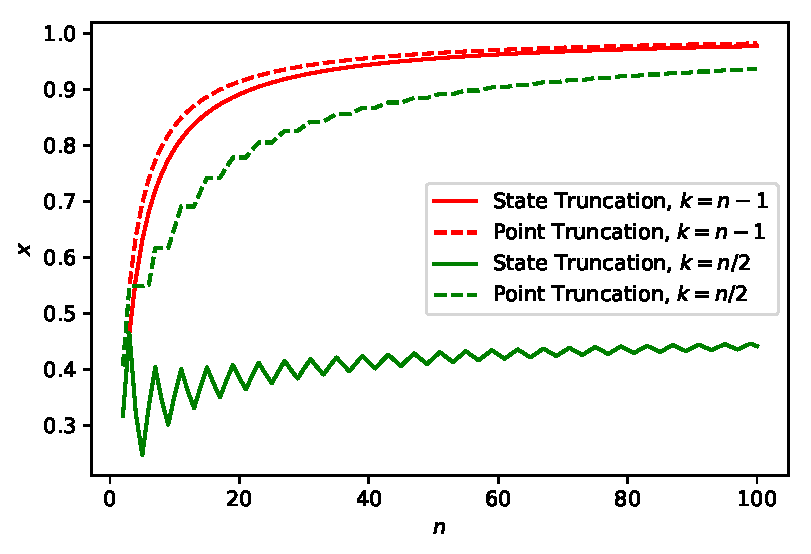
\includegraphics[width=0.45\linewidth]{classical_sim/max_x_samek}}
\hfill
\subfloat[\label{fig:max-eta-samek}]{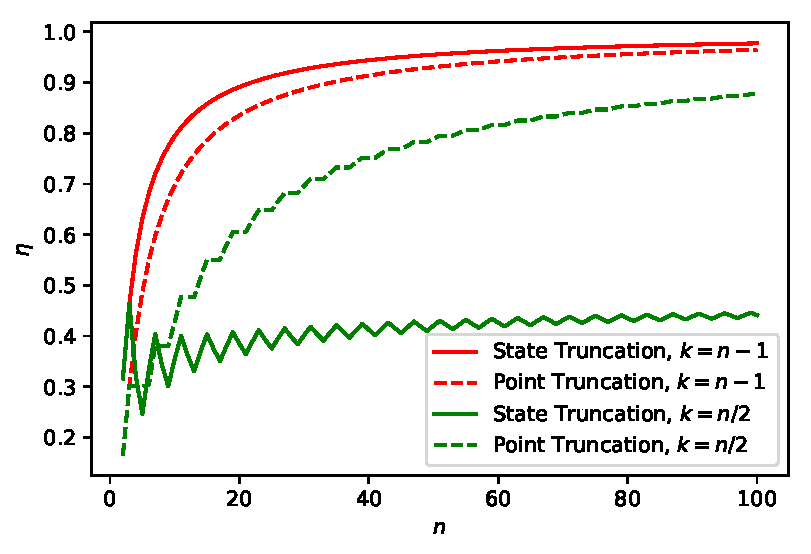
\includegraphics[width=0.45\linewidth]{classical_sim/max_eta_samek}}
\caption[Highest value of (\ref{fig:max-x-samek}) $x$ and $\eta$ simulable via state or point truncation]{\label{fig:samek} 
Highest value of (\ref{fig:max-x-samek}) $x$ when $\eta=1$ and (\ref{fig:max-eta-samek}) of $\eta$ when $x=1$ simulable via state (solid) or point (dashed) truncation up to 10\% error ($\epsilon=0.1$). 
The number of photons, $n$, is varying, with $k$ chosen as either $k=n-1$ (red) or $k=n/2$ (green).
The oscillatory behaviour is due to rounding $k=n/2$ when $n$ is odd.}
\end{figure*}

We start by comparing the performance of the two algorithms when truncated at the same level $k$. 
This is of interest as in both approaches $k$ is considered to be a parameter defining the interference between photons. 
To do so, we consider the error bounds of classically simulating $n$-photon Boson Sampling for $n$ ranging between 2 and 100. 
The values chosen for $k$ depend on $n$: we consider $k=n-1$ as the upper limit of what the two algorithms can achieve without simulating the full distribution, and also $k=n/2$ as a more feasible, though still exponential time, value.

The result is plotted in Figure \ref{fig:samek}, where in (\ref{fig:max-x-samek}) we show the highest value of $x$ simulable assuming no loss ($\eta=1$) and in (\ref{fig:max-eta-samek}) we show the highest value of $\eta$ simulable assuming the photons are fully indistinguishable ($x=1$). 
For all cases, we are considering simulations up to 10\% error.

There are a number of things we can note from Figure \ref{fig:samek}. 
First is that when $k=n-1$, we can see that both algorithms tend to the same maximum values of distinguishability and loss. 
In the case of distinguishability, we can easily see why by considering the error bounds of both algorithms. 
One can see from Equation (\ref{eqn:error-sum}) that state truncation will have a simple error bound in this case of $\epsilon \leq x^n$, meaning that for constant error the largest value of $x$ simulable is $x = \epsilon^{1/n}$. 
For point truncation, Equations (\ref{eqn:renema-variance}) \& (\ref{eqn:var}) with $k=n-1$ show that the error is similarly bounded as $\epsilon \leq x^n/\sqrt{e}$, leading to a largest value of $x=(\epsilon\sqrt{e})^{1/n}$. 
Thus, although the highest value of $x$ simulable via point truncation is higher than that via state truncation, the difference will decrease in the limit of large $n$. 
Curiously we see the same effect as well in the case of loss, but now the highest value of $\eta$ simulable via state truncation is higher than that of point truncation. 
Again, this can be shown to hold theoretically: For state truncation the error scales as $\epsilon \leq \eta^n$ according to Equation (\ref{eqn:lossy-worst}), corresponding to $\eta=\epsilon^{1/n}$; whereas for point truncation we see from Equation (\ref{eqn:renema-variance}) and substituting $x=\sqrt{\eta}$ that the error scales as $\epsilon \leq \eta^{n/2}/\sqrt{e}$, meaning a maximum value of $\eta$ is $\eta=(e\epsilon^2)^{1/n}$. 
In the limit of large $n$ these differences will also tail off.

For $k=n/2$, we see that for both distinguishability and loss point truncation is more powerful than state truncation. 
Although this is harder to formally prove, there is intuition to see why this is the case. 
For state truncation, we know that for a small error to be achievable we need $k\geq n\eta x$, as this is the mean of the binomial distribution. 
Thus for $k=n/2$, we have that $\eta x \leq 1/2$, and in both cases we see the highest value of $x$ and $\eta$ tending to a value below $1/2$. 
For point truncation on the other hand, we know that the error tends to a constant value only dependent on $k$ and $\eta x^2$ in the limit of large $n$. 
As a result, it is unsurprising that for $k$ increasing linearly with $n$ the highest values of $x$ and $\eta$ will increase.


\subsection{Comparison of runtimes}
\label{subsec:runtimes}

\begin{figure}
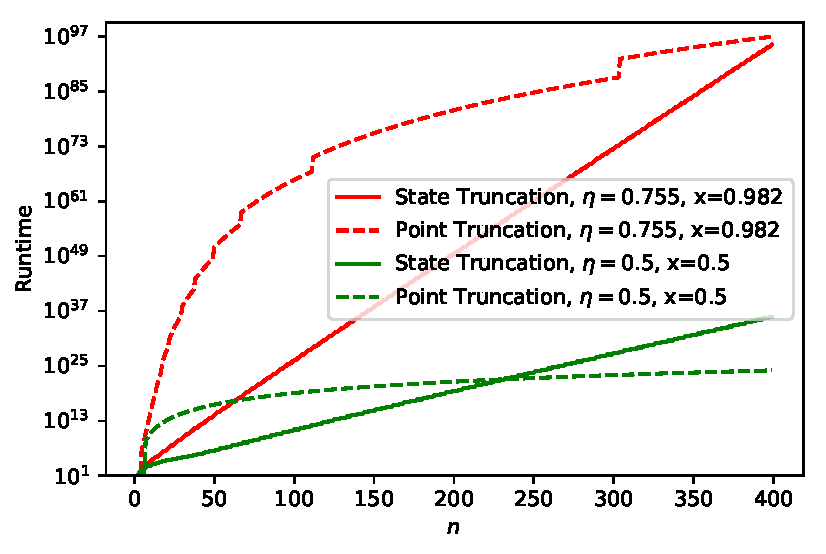
\includegraphics[width=\linewidth]{classical_sim/runtime}
\caption[Approximate runtime to simulate $n$-photon Boson Sampling with chosen values of $\eta$ and $x$ via state or point truncation]{\label{fig:runtime} Approximate runtime (number of operations) to simulate $n$-photon Boson Sampling with chosen values of $\eta$ and $x$ up to 10\% error ($\epsilon=0.1$) via state (solid) or point (dashed) truncation. Note that a modern supercomputer running for an hour can perform roughly $10^{20}$ operations.}
\end{figure}

We next consider the runtime required to simulate $n$-photon Boson Sampling up to 10\% error via either method. 
The motivation for this comparison is that the runtime of the two algorithms at the same value of $k$ are significantly different. 
In particular, the runtime of state truncation is only dependent on $k$ and not $n$, whereas the runtime for point truncation depends on a scaling of approximately $O(n^{2k})$.

To understand how the runtimes scale, in Figure \ref{fig:runtime} we plot the runtimes of classically simulating $n$-photon Boson Sampling experiments via the two approaches for fixed values of $\eta$ and $x$. 
The values of $k$ chosen for each algorithm are the smallest values for an error of at most 10\%. 
For choosing $\eta$ and $x$, we give two example cases. 
The first (Figure \ref{fig:runtime}, red), where $\eta=0.755$ and $x=0.975$, is an example of a hypothetical best experiment we could build with current technology, with the most lossless sources (82\%) \cite{slussarenko2017}, interferometers (99\%) \cite{wang2018} and detectors (93\%) \cite{marsili2013}, and the highest level of photon indistinguishability (97.6\%) \cite{he2018}. 
The second case (Figure \ref{fig:runtime}, green), where $\eta=x=0.5$, is an example of how the two algorithms perform in what would be considered a poor experiment for both distinguishability and loss. 
Actual Boson Sampling experiments are likely to fall between these two extremes.

In both cases, state truncation appears to outperform point truncation for near-term photon experiments, with point truncation eventually being able to perform faster for larger values of $n$. 
When $\eta=x=0.5$, point truncation performs better when $n$ is approximately larger than 230. 
In the case of $\eta=0.755, x=0.976$, point truncation only performs better when $n$ is approximately larger than $390$ photons. 
This gives an idea of the regions in which the polynomial runtime of point truncation can be better or worse than the exponential runtime of state truncation.

It is also worth noting that just because point truncation is faster than state truncation for large enough $n$ does not necessarily mean that either algorithm is efficient in these cases. 
When $\eta=x=0.5$, point truncation only becomes more efficient at instances where both algorithms already require the order of $10^{22}$ operations. 
And in the case where $\eta=0.755, x=0.976$, both algorithms have runtimes on the order of $10^{92}$ operations before point truncation outperforms state truncation.


\subsection{Comparison at same runtime}
\label{subsec:same-runtime}

\begin{figure*}
\subfloat[\label{fig:max-x-fixed-n-90}]{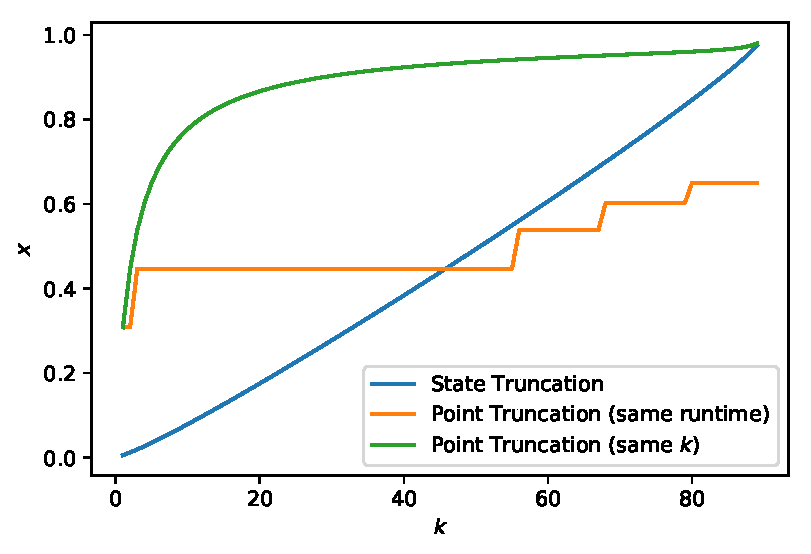
\includegraphics[width=0.45\linewidth]{classical_sim/max_x_fixed_n_90}}
\hfill
\subfloat[\label{fig:max-eta-fixed-n-90}]{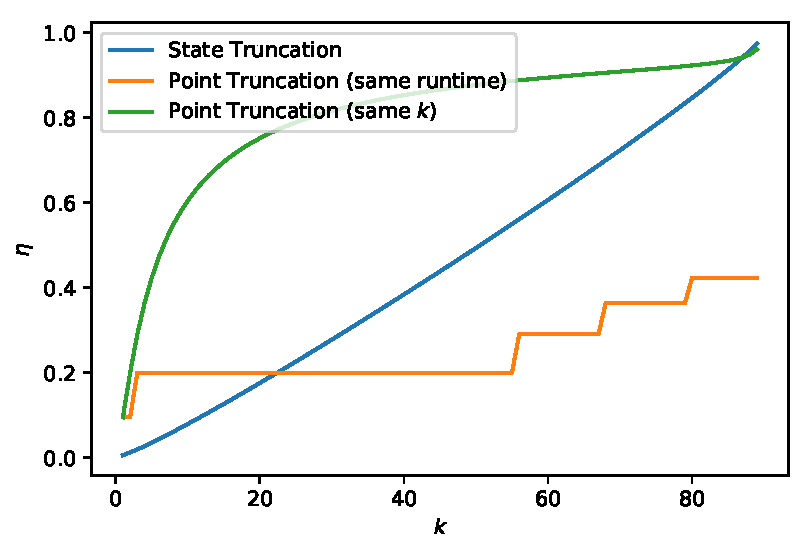
\includegraphics[width=0.45\linewidth]{classical_sim/max_eta_fixed_n_90}}
\caption[Highest value of $x$ and $\eta=1$ simulable for 90-photon boson sampling at truncation level $k$]{\label{fig:fixed-n-90} 
Highest value of (\ref{fig:max-x-fixed-n-90}) $x$ when $\eta=1$ and (\ref{fig:max-eta-fixed-n-90}) $\eta$ when $x=1$ simulable for 90-photon boson sampling at truncation level $k$ up to 10\% error ($\epsilon=0.1$). 
Blue line indicates highest values simulable via state truncation at level $k$, green lines indicate highest values simulable via point truncation at level $k$, orange lines indicate highest values simulable by point truncation at level $k'$ such that $k'$ is the smallest level of truncation such that the approximate runtime of point truncation at level $k'$ is longer than the runtime of state truncation at level $k$.}
\end{figure*}

Now we consider both truncation level and runtime, and compare the algorithms when restricted to comparable runtimes. 
To do this, we shall consider the challenge of simulating a 90-photon Boson Sampling experiment, and the largest values of distinguishability and loss that can be simulated at level $k$ with 10\% error. 
The motivation for this is that $90$ photons has been suggested as strict upper bound for what is achievable using classical computation~\cite{dalzell2018}. 

The results are shown in Figure \ref{fig:fixed-n-90}, detailing for each algorithm the highest value of $x$ simulable when $\eta=1$ (\ref{fig:max-x-fixed-n-90}) and the highest value of $\eta$ simulable when $x=1$ (\ref{fig:max-eta-fixed-n-90}). 
In both figures, the blue line indicates state truncation at level $k$, and the green line indicates point truncation at level $k$. 
However, the runtime of state truncation at level $k$ and point truncation at level $k$ are likely to be drastically different. 
To take runtime into consideration as well, we consider the orange line which indicates point truncation at level $k'$, where $k'$ is the smallest integer such that the approximated runtime of point truncation at level $k'$ is longer than that of state truncation at level $k$. 
This allows us to compare the performance of the two algorithms when restricted to similar runtimes.

Considering distinguishability in Figure \ref{fig:max-x-fixed-n-90}, we can note that point truncation with comparable runtime performs better up to $k\leq 45$, after which the methods are roughly comparable with state truncation performing marginally better, before becoming more dominant for $k\geq 60$. 
It has been suggested that boson sampling with 50 indistinguishable photons is roughly the limit of what can be classically simulated on a supercomputer \cite{neville2017, clifford2017, zhang2018}, so it appears that when considering distinguishability, the algorithms are roughly comparable in this case.

When considering loss in Figure \ref{fig:max-eta-fixed-n-90}, we see a noticeable improvement for state truncation. 
Now point truncation under the same runtime only performs better up to $k\leq 22$, with state truncation performing considerably better for higher values of $k$. 
Boson Sampling with up to 30 indistinguishable photons is already known to be classically simulable on a standard laptop \cite{neville2017}, so this appears to offer a noticeable improvement even for fast classical simulations.



\section{Non-uniform loss}

We finish by briefly considering non-uniform loss, where each photon survives a lossy optical component with probability $\tau$. 
This model of loss has been considered before \cite{garciapatron2017,oszmaniec2018}, but without the incorporation of distinguishability. We can do this using the same methods as other non-uniform loss results, by extracting non-uniform losses into a layer of uniform losses followed by a lossy interferometer. 
The uniform loss layer means that each photon has probability $\eta=\tau^s$ of surviving, where $\tau$ is the loss of each optical component and $s$ is the smallest number of lossy optical components a photon interacts with. 
If we take the total number of lossy components to be $d$, the remaining lossy circuit can be modelled as an $(m+d)$-mode interferometer, with lost photons ending up in the additional $d$ modes. 
Thus we can achieve the same error as Equation (\ref{eqn:lossy-worst}) in $O(k2^k+\poly(k,m,d))$ time. 
In typical schemes for linear interferometers, $d$ is at most polynomial in $m$ \cite{reck1994,clements2016}, so the overhead from these additional modes is small. 
We can bound the error to a decreasing value in terms of $n$ if $k>nx\tau^s$. Taking the logarithm on both sides and rearranging for $s$, we find that this holds if

\begin{equation}
s>\frac{\log n-\log 1/x-\log k}{\log1/\tau}.
\end{equation}

This matches results in \cite{garciapatron2017,oszmaniec2018}, showing that boson sampling can be classically simulated if each photon encounters at least a logarithmic number of lossy components. 
It also shows how distinguishability can affect the simulability of lossy components in Boson Sampling: if our photons are more distinguishable, corresponding to a smaller value of $x$, then we can simulate shallower (i.e.\ less total loss) optical circuits.

\section{Computing the exact trace distance}

In our analysis of the worst-case error bounds, we have simply used the property of the trace distance being convex. However, this is only an upper bound, and it could be that the actual trace distance is lower. How much can we improve this bound by more direct calculation?

Sadly there is not an easy way of calculating the exact trace distance, as we have managed to do for the fixed distinguishability cases in Section \ref{ssec:fixed-dist-distance}. In lieu of this, we use analytical code to compute the trace distance for small numbers of photons. Using symbolic programming in Mathematica, we are able to compute the exact trace distance in terms of $x$ for varying $k$ and up to four photons. Furthermore, we can use analytical programming in Matlab to produce figures plotting the trace distance over $x$ for varying values of $k$ and up to eight photons.

\section{Expanding in terms of representations}

Another natural question is if we can instead expand in terms of representations rather than in terms of state. This would provide us with an alternative decomposition where rather than needing to sample which photons are indistinguishable, we would instead be sampling an immanant to compute. It is hard to analytically work out how the different immanants contribute for general $n$, but in this section we will use results noted by Stanisic and Turner \cite{stanisic2018} to show the decompositions for two and three particles, as well as offer some general comments on why this technique might not necessarily provide a better classical simulation but could still be of theoretical interest.

We shall start with the simpler case of two photons, which we shall assume to be in the first two spatial modes. As noted earlier, the state takes the form

\begin{equation}
\rho_x = x^2\rho_{\{1,2\}} + x(1-x)(\rho_{\{1\}} + \rho_{\{2\}}) + (1-x)^2\rho_{\emptyset},
\end{equation}

\noindent where $\rho_I$ is the state corresponding to photons in modes $I\subseteq\{1,2\}$ being indistinguishable. The state corresponding to the fully indistinguishable case is fully symmetric, giving us

\begin{equation}
\rho_{\{1,2\}} = \ket{\young(12)}\bra{\young(12)},
\end{equation}

\noindent where we have suppressed notation for the irrep as it is implied by the Young tableaux, and we have suppressed the Symmetric irrep basis as it is one dimensional in the two particle cases. Note that states where only one photon is in the indistinguishable set are effectively fully distinguishable as well. As a result, all other states can be described in the irrep basis as the fully distinguishable state as given in Equation \ref{distinguishable-irreps}, giving us

\begin{equation}
\frac{1}{2}\left(\ket{\young(12)}\bra{\young(12)}+\left|\young(1,2)\right\rangle\left\langle\young(1,2)\right|\right).
\end{equation}

The overall state can therefore be written as

\begin{align}
\rho_x &= x^2\ket{\young(12)}\bra{\young(12)} + frac{(2x(1-x)+(1-x)^2)}{2}\left(\ket{\young(12)}\bra{\young(12)}+\left|\young(1,2)\right\rangle\left\langle\young(1,2)\right|\right)\\
&= \frac{1}{2}\left((2x^2 + 2x(1-x)+(1-x)^2)\ket{\young(12)}\bra{\young(12)}+(2x(1-x)+(1-x)^2)\left|\young(1,2)\right\rangle\left\langle\young(1,2)\right|\right)\\
&= \frac{1+x^2}{2}\ket{\young(12)}\bra{\young(12)}+\frac{1-x^2}{2}\left|\young(1,2)\right\rangle\left\langle\young(1,2)\right|.
\end{align}

As $x\rightarrow 1$, this tends towards only the fully symmetric irrep contributing, as expected. However, even as $x\rightarrow 0$, the fully symmetric irrep still contributes to half of the outcome probability.

We can also work out the explicit decomposition for three particles, again assuming our photons start in the first three modes. The state is now

\begin{equation}
\rho_x = x^3\rho_{\{1,2,3\}} + x^2(1-x)(\rho_{\{1,2\}}+\rho_{\{1,3\}}+\rho_{\{2,3\}}) + x(1-x)^2(\rho{\{1\}}+\rho{\{2\}}+\rho{\{3\}}) + (1-x)^3\rho_\emptyset.
\end{equation}

The fully indistinguishable state is similar to before:

\begin{equation}
\rho_{\{1,2,3\}} = \ket{\young(123)}\bra{\young(123)}.
\end{equation}

Rather than writing out the full Young-Yagamouchi basis, we shall use the same notation as in \cite{stanisic2018} to simply use a 1 or 2 subscript to denote the multiplicity of the $(1,2)$ irrep of the Unitary group. With this in mind, the uniform mixture of all three singly distinguishable states is

\begin{align}
\rho_{\{1,2\}}+\rho_{\{1,3\}}+\rho_{\{2,3\}} &= \ket{\young(123)}\bra{\young(123)} + \frac{1}{2}\left(\left|\young(12,3)_1\right\rangle\left\langle\young(12,3)_1\right| + \left|\young(12,3)_2\right\rangle\left\langle\young(12,3)_2\right|\right)\nonumber\\
&+ \frac{1}{2}\left(\left|\young(13,2)_1\right\rangle\left\langle\young(13,2)_1\right| + \left|\young(13,2)_2\right\rangle\left\langle\young(13,2)_2\right|\right).
\end{align}

Finally, we note that the fully distinguishable states can be written as

\begin{align}
&\frac{1}{6}\left(\ket{\young(123)}\bra{\young(123)} + \left|\young(12,3)_1\right\rangle\left\langle\young(12,3)_1\right| + \left|\young(12,3)_2\right\rangle\left\langle\young(12,3)_2\right|\right)\nonumber\\
&+\frac{1}{6}\left(\left|\young(13,2)_1\right\rangle\left\langle\young(13,2)_1\right| + \left|\young(13,2)_2\right\rangle\left\langle\young(13,2)_2\right| + \left|\young(1,2,3)\right\rangle\left\langle\young(1,2,3)\right|\right).
\end{align}

The overall state can be expanded as

\begin{align}
\rho_x &= \frac{1}{6}\left((1+3x^2+2x^3)\ket{\young(123)}\bra{\young(123)} + (1-x^3)\left(\left|\young(12,3)_1\right\rangle\left\langle\young(12,3)_1\right| + \left|\young(12,3)_2\right\rangle\left\langle\young(12,3)_2\right|\right)\right)\nonumber\\
&+\frac{1}{6}\left((1-x^3)\left(\left|\young(13,2)_1\right\rangle\left\langle\young(13,2)_1\right| + \left|\young(13,2)_2\right\rangle\left\langle\young(13,2)_2\right|\right) + (1-3x^2+2x^3)\left|\young(1,2,3)\right\rangle\left\langle\young(1,2,3)\right|\right).
\end{align}

It is again possible to verify that as $x\rightarrow 1$ then only the symmetric irrep contributes, and as $x \rightarrow 0$ then all irreps contribute uniformly.

\begin{figure}
\subfloat[\label{fig:irreps-n-2}]{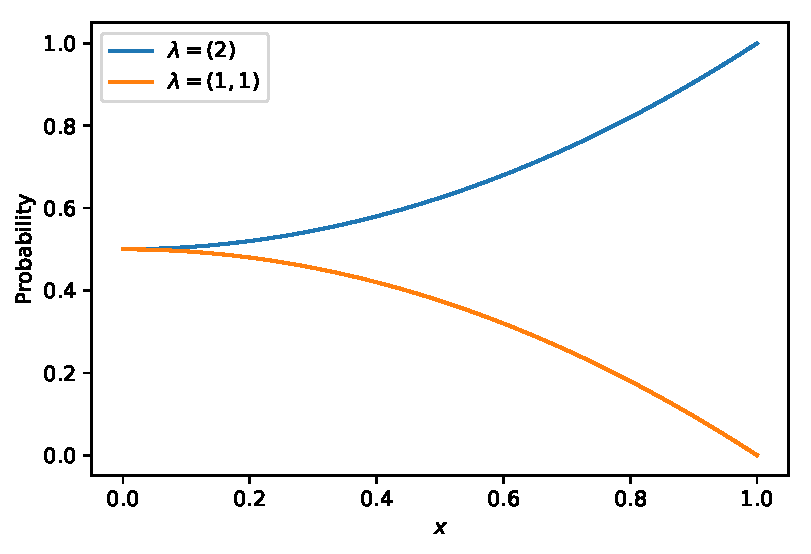
\includegraphics[width=0.45\linewidth]{classical_sim/irreps_n_2}}
\hfill
\subfloat[\label{fig:irreps-n-3}]{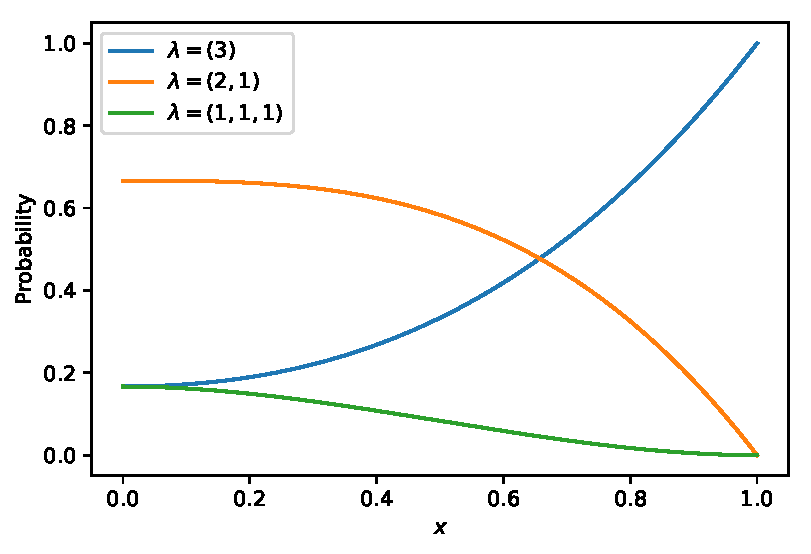
\includegraphics[width=0.45\linewidth]{classical_sim/irreps_n_3}}
\caption[Probability of different irreps when $n=2$ and $n=3$.]{\label{fig:irreps} Probability of different irreps when (\ref{fig:irreps-n-2}) $n=2$ and (\ref{fig:irreps-n-3}) $n=3$. Note that if for the $\lambda=(2,1)$ irrep in Figure \ref{fig:irreps-n-3}, we have shown the probability of sampling any of the multiplicities, when in reality this is a uniform distribution of the four multiplicities.}
\end{figure}

In Figure \ref{fig:irreps} we have plotted the probability of sampling from different irreps over $x \in [0,1]$ for (\ref{fig:irreps-n-2}) $n=2$ and (\ref{fig:irreps-n-3}) $n=3$. As already mentioned, this makes clear how at $x=0$ all terms have equal probability, and as $x\rightarrow 1$ the fully symmetric irrep begins to dominate. It is interesting to note that for $n=3$, $\lambda=(2,1)$ is the most likely irrep; this is because of the multiplicities within this irrep for both $\symm_3$ and $\unitary(3)$. By solving the cubic equation

\begin{equation}
1+3x^2+2x^3 = 4-4x^3,
\end{equation}

\noindent we find that the two overlap when $x \approx 0.657$, when both irreps have probability approximately $0.4773$ of being sampled\footnote{Note that there are other solutions to this cubic equation, but $x\approx 0.657$ is the only real-valued solution between 0 and 1 and is therefore the only solution relevant to us.}.

We now go back to the question at the start of this section, as to whether or not this could lead to another simulation. A potential method of simulation, akin to the point and state truncation methods, would be to truncate which irrep we sample from. In other words, we sample an irrep with at most $n-k$ nonzero rows for some truncation level $k$, and then perform sampling conditioned on that irrep.

There are a few limitations with this approach. The first is that this expansion is nontrivial, and we do not currently have a convenient general form for it, unlike with state truncation where we simply follow the binomial distribution. The second is that, even in the fully distinguishable case, the matrix permanent still plays a role in the distribution, so for any value of $x$ including $x=0$ we are going to have some error if we truncate before the symmetric irrep. And the third is that it is unclear how to classically simulate these irrep states under unitary action; it seems reasonable for them to be related to matrix immanants in some way \`{a} la Tichy and M\o lmer \cite{tichy2017}, but even if so classical algorithms for computing more general immanants are less well-known, though some do exist \cite{hartmann1985, barvinok1990, burgisser2000}. Obviously classical algorithms for the special cases of the permanent and determinant are well-known with exponential \cite{glynn2010} and polynomial \cite{fisikopoulos2016} runtimes, respectively.

So if this decomposition does not provide us with faster classical algorithms, what might it be useful for? Well, there are some instances of $\lambda$ for which matrix imminants are known to be hard. The best-known of these is the permanent \cite{valiant1979, aaronson2011}, but other forms of immanant are also know to be $\#P$-hard \cite{hartmann1985, burgisser2000, brylinski2003, mertens2013}. If one is able to construct a form of distinguishable-photon Boson Sampling such that the probability ends up being largely concentrated in these hard instances, and show that computing the sum of these immanants is at least as hard as computing a single immanant, then this could potentially lead to new proofs of hardness for Boson Sampling under distinguishability. We leave this question as future work.

\section{Conclusion}
\label{sec:conclusion}

In recent years significant improvements have been made in the ability of classical computers to simulate Boson Sampling under various imperfections. 
However, while it is of theoretical interest to demonstrate asymptotic improvements in classical simulation, the whole reason for proposals such as Boson Sampling is to offer speedups for near-term devices. 
Although our algorithm will not scale polynomially as the number of photons increases, we find that a substantial improvement over current classical algorithms can be achieved for the numbers of photons that experimentalists are currently aiming for. 
In doing so, we have effectively set a benchmark for what is required of a 50-90 photon Boson Sampling device.

There are a number of ways one could improve this classical simulation. 
In particular, the approach of Ref.~\cite{renema2018} for truncation when looking at near-term devices is dependent on Metropolised Independence Sampling. 
A direct adaptation of the Clifford \& Clifford algorithm to this approach would almost certainly offer an improvement over our algorithm. 
However, such an adaptation is non-trivial, due to the fact that the term in the expansion are not states, something that motivated our work here.

There are other open questions we would like to consider as well. The first would be to reduce the average-case error bounds to be less than our worst-case error bounds. This would most likely involve an alternative to using the triangle inequality. The second would be to find a way of explaining the difference in dependence on $\eta$ and $x$ between point and state truncation, and ideally improving either algorithm in the process.


\subsection{Note Added}

During this work we were made aware of independent work by V. Shchesnovich, which also shows that the model of distinguishability considered by Renema et al.\ corresponds to that of selecting indistinguishable photons via the binomial distribution \cite{shchesnovich2019}. 
This is derived using significantly different methods from those used in this manuscript, and does not consider classical simulation of distinguishability via the above method (though this has been anticipated~\cite{shchesnovich2019clifford}).

No underlying data was produced during this study.